\hypertarget{experimental-setup}{%
\chapter{Experimental setup}\label{experimental-setup}}

As stated previously, the core work of this thesis is performing N-body
simulations of the infall of Sgr in the style of Dierickx et
al.~\cite{dierickx_predicted_2017}, varying the initial conditions and dark
matter model to determine the resulting impacts on the evolution of the Sgr
tidal debris stream. As such, we provide an overview of the simulations we
performed in this section.

\hypertarget{pipeline-and-parameters}{%
\section{Pipeline and parameters}\label{pipeline-and-parameters}}

To begin our experimental pipeline, we first generate the initial
distributions of stellar and dark matter particles using a package called
GalactICS~\cite{deg_galactics_2019}. Each galaxy is model using a tellar disk
and dark matter halo. The halo follows a Navarro-Frenk-White (NFW) profile
\begin{equation}
    \rho_{\text{halo}} (r) = 
    \frac{M_{200}}{4\pi a^3 f(c)} 
    \frac{1}{(r/a)(1+r/a)^2},
\end{equation}
where $f(c) = \log (1+c) - c/(1+c)$, $M_{200}$ is the virial mass, $a$ is the
scale length, $c$ is the concentration, and $c = r_{200} / a$. Here, we use a
lowercase $r$ to denote the radius in a spherical sense.

The stellar disk follows an exponential-sech$^2$ profile, given by
\begin{equation}
    \rho_{\text{disk}} (R, z) = 
    \frac{M_{\text{disk}}}{4 \pi R_0^2 z_0}
    \exp(-R/R_0) \text{ sech}^2(z/z_0),
\end{equation}
where $R_0$ is the disk scale length, $z_0$ is the disk scale height, and the
capital $R$ denotes the cylindrical radius in the plane of the disk.

Both of these distributions are subject to truncation beyond a certain
radius, \(r_t\), with truncation width \(dr_t\). The truncation function
comes from~\cite{widrow_dynamical_2008} and is given by
\begin{equation}
C(r; r_t, dr_t) = \frac{1}{2} \text{erfc} 
\left( \frac{r - r_t}{\sqrt{2} dr_t} \right).
\end{equation}
For the halos, the truncation radius is simply the virial radius and the
truncation width is 20 kpc. For the disks, the truncation radius is 25 kpc,
the width is 5 kpc, and the truncation is only applied to $R$ in the disk
plane. The distributions, including the truncation parameter, can be seen in
Figure~\ref{fig:init_profiles}.

\begin{figure}
    \centering
    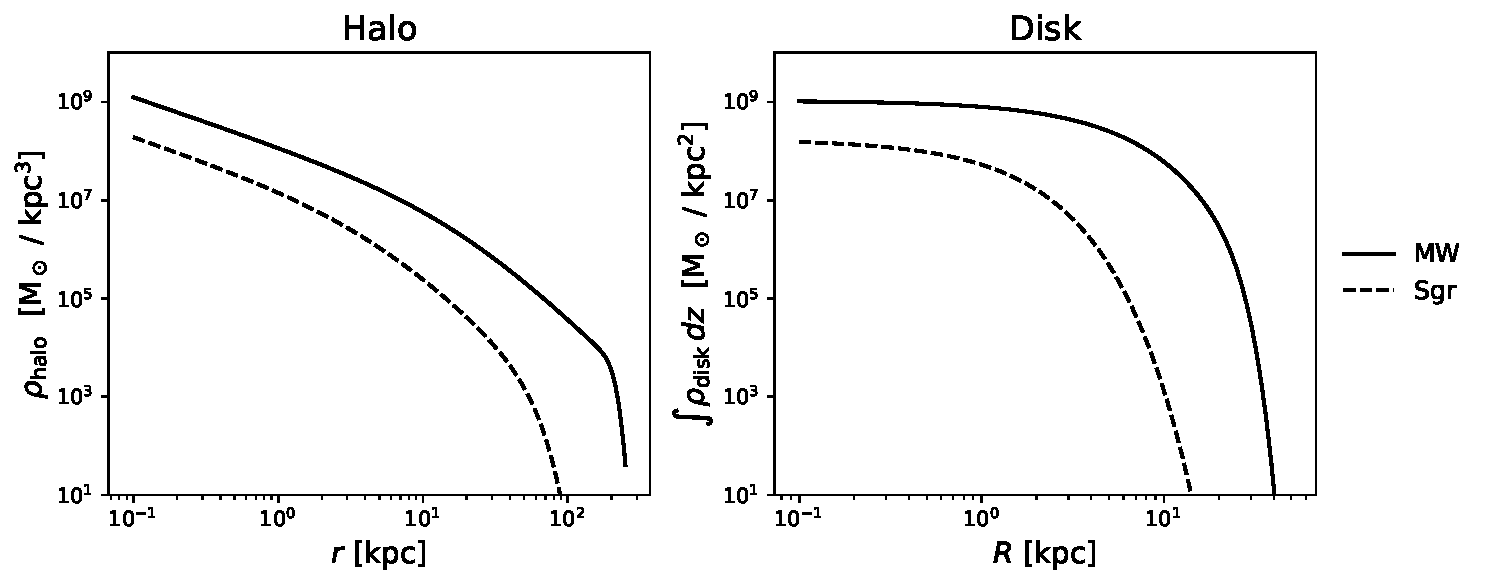
\includegraphics[width=0.9\linewidth]{figs/init_profiles.pdf}
    \caption{%
        Initial profiles for the halo and disk of both galaxies. The halos
        follow a truncated NFW profile and the disks follow a truncated
        exponential-sech$^2$ profile. Note that the disk density is in
        cylindrical coordinates and is integrated over the $z$ direction.
    }
    \label{fig:init_profiles}
\end{figure}

Bundled with GalactICS is a subpackage called GadgetConverters, which
provides a pipeline for converting the native output of GalactICS into a
binary compatible with GADGET and derivative N-body simulation software. In
this work, we use GIZMO~\cite{hopkins_new_2015}, which is itself derived from
GADGET-2~\cite{springel_cosmological_2005}.

\begin{table}
\centering
\begin{tabular}{lcll}
    \toprule
    Parameters & & MW & Sgr \\
    \midrule 
    Halo virial mass & $M_{200}$ & $10^{12}$ M$_\odot$ & $10^{10}$ M$_\odot$ \\
    Halo virial radius & $R_{200}$ & 206 kpc & 44 kpc \\
    Halo concentration & $c$ & 10 & 8 \\
    Halo particles & $N_{\text{halo}}$ & $1.16 \times 10^{6}$ & $1.17 \times 10^{4}$ \\
    Disk mass & $M_{\text{disk}}$ & $6.5 \times 10^{10}$ M$_\odot$ & $6 \times 10^{8}$ M$_\odot$ \\
    Disk scale length & $b_0$ & 3.5 kpc & 0.85 kpc \\
    Disk scale height & $c_0$ & 0.53 kpc & 0.13 kpc \\
    Disk truncation radius & $r_{\text{trunc}}$ & 25 kpc & 25 kpc \\
    Disk particles & $N_{\text{disk}}$ & $2.03 \times 10^{6}$ & $1.17 \times
    10^{4}$ \\
    \bottomrule
\end{tabular}
\caption{%
    Parameters for the initial Milky Way and Sgr galaxies in our full
    simulation. These values are in large part taken from the work
    of~\cite{dierickx_predicted_2017}.
}
\label{tab:sim_params}
\end{table}

The parameters that were used for our simulations were largely taken from the
work of Dierickx et al.~\cite{dierickx_predicted_2017}. They are summarized in
Table~\ref{tab:sim_params}. There are a few key differences between their model
and our simulations, however. First, they used Hernquist profiles for their
halos, while we use NFW distributions. The NFW parameters we use, however, come
from their work, listed as the approximately equivalent NFW distributions. A
comparison between their Hernquist and our NFW profiles is shown in
Figure~\ref{fig:nfw_vs_hernquist}; the differences are quite small.

\begin{figure}
    \centering
    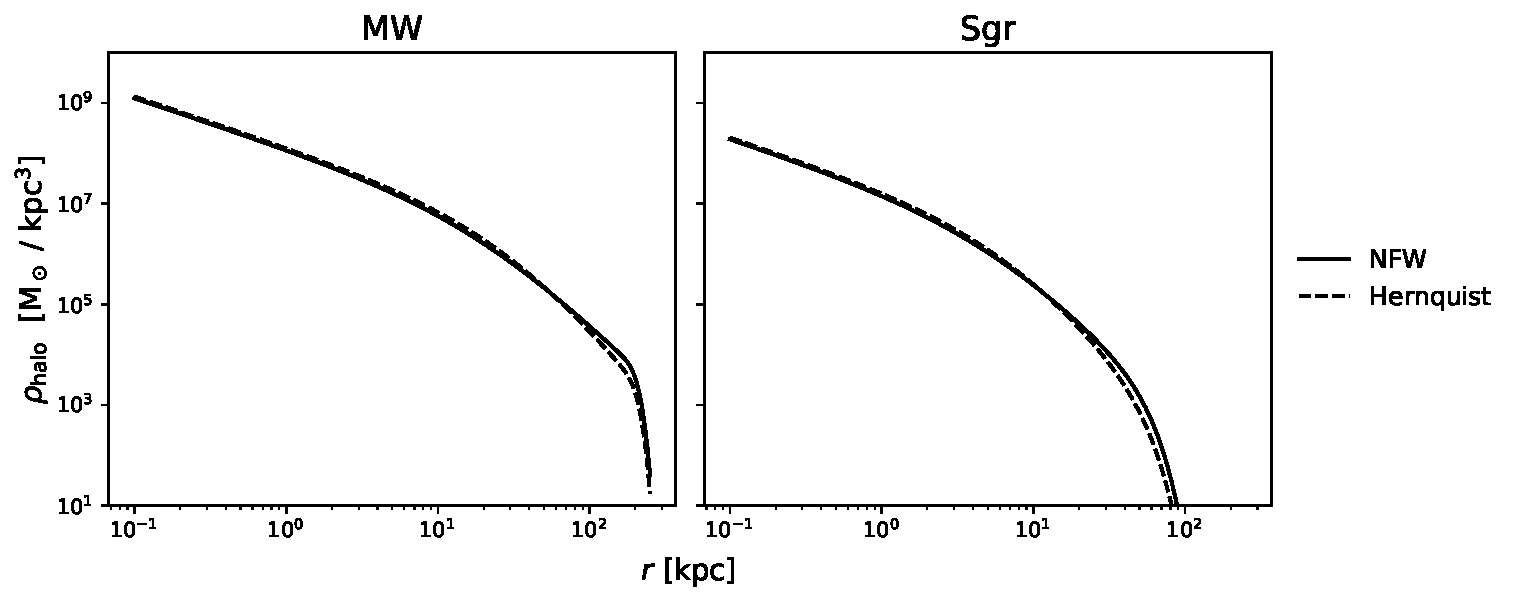
\includegraphics[width=0.9\linewidth]{figs/nfw_vs_hernquist.pdf}
    \caption{%
        Comparison between the density profiles of the relevant truncated NFW
        and truncated Hernquist profiles for the Milky Way and Sgr galaxies in
        the Dierickx model.
    }
    \label{fig:nfw_vs_hernquist}
\end{figure}

The second source of discrepancy between their work and ours is that we have
less resolution in our stellar profile than in their work. This is in part
because they used a Hernquist bulge in both their Milky Way and Sgr, wherer this
has been omitted from our work. It is also because they used more stellar
particles for the Sgr disk than we did ($1.94 \times 10^4$ versus $1.17 \times
10^4$), owing to a technical error in our initial conditions creation
pipeline.

The experiments performed herein were performed using GIZMO version
(todo find out) on Princeton Research Computing's Della cluster. This
cluster is an Intel cluster with $\geq 20$ cores per node and $\geq
128$ GB memory per node~\cite{princeton_research_computing_della_nodate}. Our
simulations often required several dozen gigabytes of RAM and typically split
the computation over many (todo how many) cores.

\hypertarget{equilibration}{%
\section{Equilibration}\label{equilibration}}

After generating the initial particle distributions for each galaxy, we
evolved each one forward in time for a several Gyr to allow it to
equilibrate. For our runs involving SIDM, we perform this equilibration
run with SIDM microphysics turned on, allowing for the creation of a
core in the central region of the dark matter halo.

For each galaxy, we begin with the parameters discussed in the previous
section and perform two equilibration runs: one using CDM microphysics
and one using SIDM microphysics with a cross section of
\(\sigma / m = 10\) cm\(^2\)/g. In this study, we choose to use a
somewhat high cross section in order to exaggerate any differences that
may appear because of the presence of self-interaction. We note that
future studies should consider a range of cross sections.

For the Milky Way equilibrations---both CDM and SIDM---we only evolve
the galaxy forward for 2 Gyr, writing time stamps approximately every
0.1 Gyr. This is because we expect the initial distribution to be
relatively close to equilibrium, especially when considering such a
large galaxy. The resulting evolution of the mass density profiles are
shown in Figure todo.

todo add figure of mw eq mass density evolution todo add discussion of
mw eq mass density evolution todo try to apply SIDM analytic description
here

For the Sgr equilibrations, however, we evolved the galaxy much farther
forward in time: approximately 10 Gyr for the CDM case and 20 Gyr for
SIDM. These evolution times do not correspond to a physical orbit
(especially given that the SIDM case would exceed the lifetime of the
Universe). Rather, the initial Sgr distribution was found to be a bit
unstable. We also wanted to be absolutely certain that the SIDM case
would develop a cored profile. The evolution of the resulting Sgr mass
profiles is shown in Figure todo.

todo add figure of sgr eq mass density evolution todo add discussion of
sgr eq mass density evolution todo try to apply SIDM analytic
description here

more discussion

With the equilibrated MW and Sgr galaxies in both the cuspy and cored
régimes, we combine them to give us two initial conditions for mergers:
cuspy and cored. The Milky Way is left at its position from the
equilibration run, as its center of mass will be close to the origin and
its net velocity will be close to zero. Sgr is placed such that its
center of mass lies at the point \([125, 0, 0]\) and is given an initial
velocity \([-10,0,70]\). These values correspond to the best fit values
found in~\cite{dierickx_predicted_2017}.
